\documentclass[conference]{IEEEtran}
\IEEEoverridecommandlockouts
% Fix margins and standard packages
\usepackage{cite}
\usepackage{amsmath,amssymb,amsfonts}
\usepackage{algorithmic}
\usepackage{graphicx}
\usepackage{textcomp}
\usepackage{xcolor}
\usepackage{booktabs}
\usepackage{multirow}
\usepackage{url}
\usepackage{microtype}

\def\BibTeX{{\rm B\kern-.05em{\sc i\kern-.025em b}\kern-.08em
    T\kern-.1667em\lower.7ex\hbox{E}\kern-.125emX}}

\begin{document}

\title{Bhu-Overlay: An AI-Augmented Cadastral GIS Platform with Deterministic Spatial Geometry and Statutory Land Partitioning}

\author{\IEEEauthorblockN{Karthikeyan A}
\IEEEauthorblockA{\textit{School of Computer Science and Engineering} \\
\textit{Vellore Institute of Technology}\\
Vellore, Tamil Nadu, India \\
karthikeyan.a2023@vitstudent.ac.in}
\and
\IEEEauthorblockN{Vishal B}
\IEEEauthorblockA{\textit{School of Computer Science and Engineering} \\
\textit{Vellore Institute of Technology}\\
Vellore, Tamil Nadu, India \\
vishal.b2023@vitstudent.ac.in}
}

\maketitle

\begin{abstract}
Agricultural land fragmentation and inheritance disputes present severe administrative bottlenecks across developing rural economies. In the Indian agrarian context, the statutory division of agricultural holdings---termed \textit{Kurra} partition under the Revenue Code---relies predominantly on manual field measurements by revenue surveyors using brass chains and ocular estimations. This manual paradigm frequently produces landlocked sub-parcels, inequitable road frontage allocation, and protracted judicial litigation. This paper introduces \textbf{Bhu-Overlay}, a lightweight, full-stack cadastral Geographic Information System (GIS) and statutory land partition platform engineered for rural land administration. The system integrates official government cadastral web services (BhuNaksha) with high-resolution satellite imagery via an on-demand reverse proxy and local spatial caching layer. We present a deterministic computational geometry engine that handles non-convex, multi-vertex cadastral boundaries, automatically resolves boundary self-intersections, and performs iterative swept-plane bisections to satisfy arbitrary co-sharer ratios with absolute area conservation (error $< 0.005\%$). To ensure equitable land partition, candidate partition topologies are evaluated across quantitative compactness ($4\pi A / P^2$), infrastructure frontage parity, and localized feature preservation (trees and irrigation wells). A large language model (LLM) advisory layer grounded in statutory provisions (Sections 116--117 and Rule 109 of the Revenue Code) ranks candidate divisions and synthesizes legal recommendations, supported by a deterministic mathematical fallback for offline field deployment. Experimental validation on 70 official cadastral parcels from Bihar demonstrates sub-50\,ms partition computation, complete area preservation, and automated generation of statutory vector survey reports.
\end{abstract}

\begin{IEEEkeywords}
Cadastral GIS, Land Partitioning (Kurra), BhuNaksha, Computational Geometry, Shapely, Statutory Legal Compliance, Large Language Models, Revenue Administration.
\end{IEEEkeywords}

\section{Introduction}
Secure property boundaries and transparent land tenure are fundamental prerequisites for agricultural productivity, credit access, and rural economic growth \cite{deininger2003land}. In India, land records have historically suffered from structural fragmentation resulting from generational succession, unrecorded sub-divisions, and imprecise paper maps known as \textit{khasra} and \textit{shajra} (cadastral sheets). Although initiatives under the Digital India Land Records Modernization Programme (DILRMP) have digitized cadastral parcel boundaries via state-level portals such as BhuNaksha \cite{national2021dilrmp}, the operational application of these digital maps for statutory field disputes remains hindered by significant technical and procedural barriers.

The primary legal mechanism for resolving co-tenancy disputes is the partition of agricultural holdings, codified under the State Revenue Codes (such as Sections 116 and 117 of the Uttar Pradesh and Bihar Revenue Codes). In this statutory process, revenue courts mandate the preparation of \textit{Kurra} (allotment of independent, demarcated plots to co-owners according to their respective shares). In customary field practice, the revenue surveyor (\textit{Ameen}) visually inspects the parcel, measures boundary perimeters using metric chains (\textit{jarib}), and draws partition lines on tracing cloth. This conventional workflow exhibits three chronic failure modes:
\begin{enumerate}
    \item \textbf{Inequitable Infrastructure Allocation:} Sub-parcels are routinely created without direct access to village thoroughfares, public roads, or irrigation canals, rendering interior tracts landlocked and economically unviable.
    \item \textbf{Irregular Shape Factor and Boundary Tortuosity:} Manual splits produce acute sliver polygons, disproportionate perimeter-to-area ratios, and uncultivable border strips that infringe upon statutory compactness guidelines.
    \item \textbf{Sub-Surface Asset Disputes:} Immovable micro-assets, including mature fruit-bearing trees, tube-wells, and field channels, are often bisected or disproportionately assigned, triggering appeals that congest revenue courts for decades \cite{wadhwa2002guaranteeing}.
\end{enumerate}

To bridge the gap between static cadastral databases and actionable, dispute-free field partitioning, we develop and evaluate \textbf{Bhu-Overlay}. The system unites web-based geospatial layers, deterministic polygon bisection algorithms, live road/river infrastructure extraction, and an automated statutory compliance reasoning agent.

The principal technical contributions of this study are:
\begin{itemize}
    \item A resilient \textbf{cadastral integration pipeline} that reverse-engineers BhuNaksha REST endpoints and dynamic Web Map Services (WMS), incorporating dynamic SSL bypass proxies, coordinate transformations (WGS84 to UTM Zone 45N), and an offline-first SQLite spatial database caching parcel polygons and administrative hierarchies.
    \item A \textbf{deterministic geometric partitioning engine} based on computational geometry primitives that guarantees exact area conservation across arbitrary co-sharer fractions, automatically rectifies self-intersecting boundary polygons, and constructs multiple topologically distinct subdivision candidates (compact transverse cuts, longitudinal splits, and road-frontage-aligned partitions).
    \item An \textbf{infrastructure-aware and feature-preserving objective function} that ingests live government ArcGIS vector layers (highways, village roads, river paths) and user-demarcated micro-assets (trees, borewells) to calculate objective access scores for each generated sub-parcel.
    \item A \textbf{statutory LLM reasoning engine} powered by Google Gemini that inspects parcel aspect ratios, frontage metrics, and local assets against codified legal principles (such as Rule 109 compactness and equality of soil valuation) to provide an authoritative, auditable partition decree accompanied by automated vector PDF report generation.
    \item A comprehensive \textbf{empirical benchmark} evaluated on 70 official cadastral sheets from Bihar, India, establishing end-to-end computational throughput, zero area degradation, and deterministic offline fallback reliability.
\end{itemize}

\section{Related Work}

\subsection{Cadastral Systems and Cadastral Digitization}
Cadastral records represent the legal and spatial foundation of property ownership worldwide. Classical cadastral systems categorized land primarily through metes and bounds descriptions or graphic paper maps \cite{dale1999cadastral}. The advent of modern Spatial Data Infrastructures (SDIs) catalyzed the transition toward vector-based cadastre, enabling spatial indexing, topological validation, and web dissemination through Open Geospatial Consortium (OGC) standards \cite{rajabifard2006spatially}. In India, the National Informatics Centre (NIC) deployed BhuNaksha, an open-source cadastral mapping solution implemented on GeoTools and PostgreSQL/PostGIS. While BhuNaksha enables web-based viewing and Land Parcel Map (LPM) generation, it operates as a centralized, read-only system lacking automated land subdivision optimization, spatial multi-criteria evaluation, or interactive co-tenancy arbitration tools.

\subsection{Polygon Decomposition and Spatial Subdivision}
The problem of dividing a polygon into specified area ratios has extensive precedents in computational geometry, architectural space planning, and cartographic generalization \cite{de2000computational}. Early theoretical approaches addressed convex polygon bisection using rotating swept lines and Hamiltonian paths. Extending bisection to arbitrary simple non-convex polygons requires rigorous handling of reflex vertices and fragmented intersections \cite{lingas1982convex}. 

In spatial economics and urban layout synthesis, Voronoi tessellation variants---such as Centroidal Voronoi Tessellations (CVT) and Power Diagrams (Laguerre tessellations)---are widely employed to generate bounded land parcels \cite{araujo2014automated}. However, Voronoi-based decomposition methods inherently optimize toward point centroids rather than adhering to rigid agricultural boundary constraints, often yielding curved or multi-faceted segment lines that are impossible to survey or fence on real rural terrain. Consequently, swept-line bisection aligned to principal parcel axes remains the golden standard for practical boundary demarcation.

\subsection{Artificial Intelligence in Legal Reasoning and GIS}
The convergence of spatial computing and Large Language Models (LLMs) has opened new frontiers for automated statutory compliance and spatial governance \cite{mai2023opportunities}. Traditional automated legal systems relied on hardcoded rule engines, propositional logic trees, and expert knowledge graphs \cite{sergot1986british}. Although deterministic, symbolic rule engines struggle with qualitative statutory clauses that mandate ``equitable access,'' ``convenient agricultural shape,'' or ``protection of shared improvements.'' 

Recent work demonstrates that prompt-engineered LLMs with structured outputs can interpret statutory codes and evaluate multi-variable decision matrices \cite{katz2024gpt}. However, deploying generative models in legal and administrative contexts introduces hallucination risks and computational fragility. Bhu-Overlay mitigates these risks by separating deterministic geometric computations from the linguistic reasoning layer, using the LLM strictly to evaluate structured spatial metrics against codified statutes, reinforced by a zero-shot deterministic fallback.

\begin{figure*}[!t]
\centering
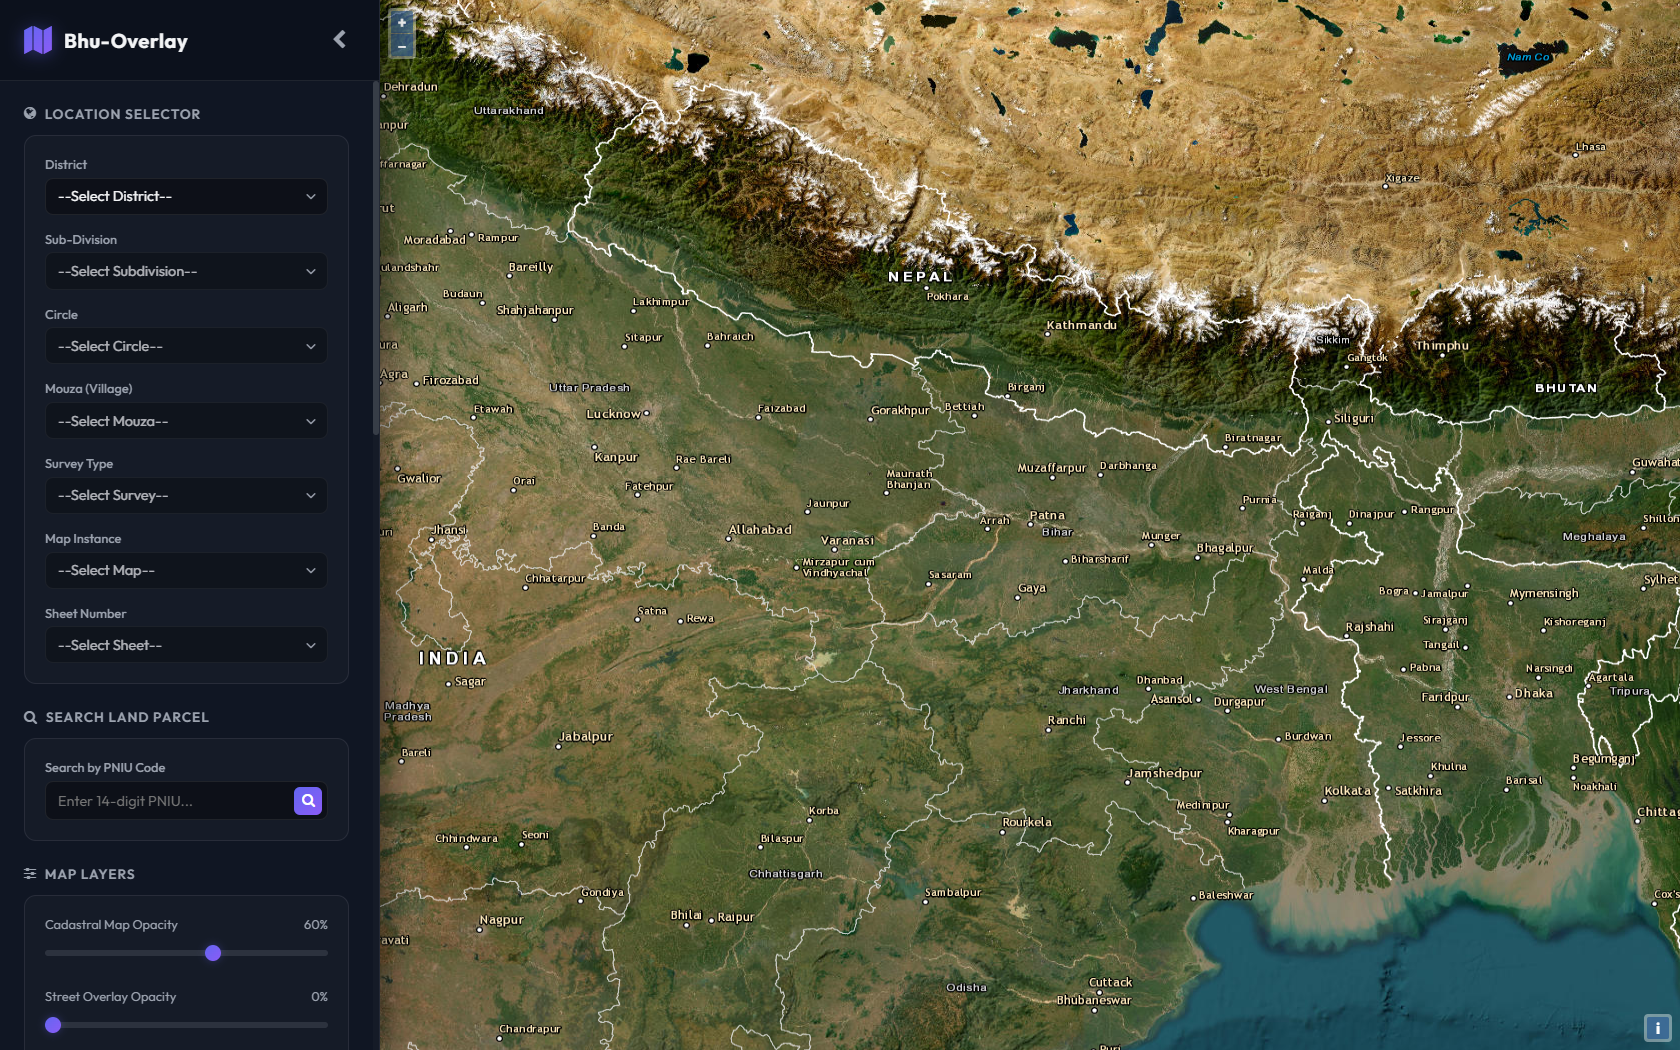
\includegraphics[width=0.98\textwidth]{docs/screenshots/bhu_01_dashboard_initial.png}
\caption{Architectural overview and runtime user interface of the Bhu-Overlay platform. The interface combines an interactive OpenLayers v6 GIS canvas with ArcGIS World Imagery, an administrative 7-tier cascading hierarchy selector (District, Sub-Division, Circle, Mouza, Survey, Map, Sheet), an opacity-controlled BhuNaksha cadastral tile overlay, real-time parcel metric analytics, and the interactive Kurra subdivision suite.}
\label{fig:dashboard_overview}
\end{figure*}

\section{System Architecture and Data Pipeline}

The overall architecture of Bhu-Overlay is structured into a lightweight, modular three-tier pipeline: client-side spatial presentation, backend routing and proxy orchestration, and computational geometry coupled with statutory reasoning. Fig.~\ref{fig:dashboard_overview} displays the production web dashboard.

\subsection{Client-Side Spatial Interface}
The client is implemented as a single-page web dashboard using OpenLayers v6 and Vanilla CSS. The map engine maintains five synchronized spatial layers:
\begin{enumerate}
    \item \textbf{High-Resolution Basemap:} Hybrid ArcGIS World Imagery (Level 17 maximum zoom) coupled with reference transport and place labels, switchable to standard vector street basemaps.
    \item \textbf{Government Cadastral Layer (\textit{plotLyr}):} Dynamically proxied BhuNaksha WMS tiles rendered with transparency sliders to enable overlay visual inspection.
    \item \textbf{Cadastral Inspection Layer (\textit{vectorLayer}):} An interactive OpenLayers Vector source rendering the exact geometry of the queried plot, displaying boundary vertices as high-contrast nodes and annotating individual edge lengths directly on the canvas.
    \item \textbf{Kurra Partition Layer (\textit{kurraVectorLayer}):} Dynamically styled sub-parcel polygons rendered with categorical fills and centroid identifiers.
    \item \textbf{Micro-Asset Layer (\textit{osmVectorLayer}):} Vector markers representing manual field overrides placed by surveyors, such as mature trees, borewells, or boundary stones.
\end{enumerate}

\subsection{Government GIS Proxy and Reverse Geocoding}
Direct client-side consumption of state cadastral portals is infeasible due to strict Cross-Origin Resource Sharing (CORS) policies, variable SSL certificate authorities, and non-standard JSON/XML payload schemas. The Flask backend implements an asynchronous reverse proxy layer that manages:
\begin{itemize}
    \item \textbf{Session Cookie Synchronization:} Automatically initializes and preserves ASP.NET and JSESSIONID state cookies in \texttt{data/session\_cookies.json}.
    \item \textbf{Dynamic Coordinate Transformations:} Government BhuNaksha instances alternate between local UTM projections and geographic GPS coordinates ($\text{EPSG:4326}$). The proxy ingests raw spatial responses, detects coordinate frame anomalies (e.g., coordinates exceeding $180^\circ$ indicating metric UTM), and normalizes bounding boxes.
    \item \textbf{Click-to-Parcel Reverse Geocoding:} When a user clicks any coordinate $(lon, lat)$ on the satellite canvas, the backend transforms the coordinate to local projection space and queries both the local SQLite cache and the upstream REST service:
    \begin{equation}
        (x_{\text{utm}}, y_{\text{utm}}) = \mathcal{T}_{\text{EPSG:4326} \to \text{EPSG:32645}}(lon, lat)
    \end{equation}
    returning the matching cadastral plot identifier (\textit{kide}) in sub-100\,ms.
\end{itemize}

\subsection{Offline-First SQLite Spatial Caching}
To support rural deployment where field connectivity is intermittent, the platform integrates an embedded SQLite persistence layer (\texttt{data/app.db}). The schema maintains normalized entities for parcels, boundary vertices, side segments, and generated legal decrees. Once a cadastral sheet is scraped or an individual plot is inspected, its topological vertices and metadata are cached locally. Subsequent inspections, geometry queries, and partition requests execute directly against local SQLite storage, eliminating external network dependencies.

\section{Deterministic Computational Geometry Engine}

The core partitioning module is implemented in \texttt{backend/geometry.py} using the Shapely library (backed by GEOS). The mathematical workflow guarantees strict area conservation, shape regularity, and topological validity.

\subsection{Boundary Repair and Metric Calculation}
Cadastral polygons digitized from legacy village maps frequently contain topological anomalies, including self-intersecting loops, colinear sliver vertices, and duplicate closing coordinates. Prior to geometric analysis, each raw polygon $\mathcal{P}_{\text{raw}}$ undergoes topological normalization:
\begin{equation}
    \mathcal{P} = \begin{cases}
        \mathcal{P}_{\text{raw}}, & \text{if } \text{isValid}(\mathcal{P}_{\text{raw}}) \\
        \text{Buffer}(\mathcal{P}_{\text{raw}}, 0), & \text{otherwise}
    \end{cases}
\end{equation}
The zero-width buffer operation reliably decomposes complex bow-tie polygons into clean multi-polygons, from which the maximal contiguous exterior shell is retained.

For an $N$-vertex polygon $\mathcal{P} = \{(x_0, y_0), (x_1, y_1), \dots, (x_{N-1}, y_{N-1})\}$, exact area $A(\mathcal{P})$ and perimeter $P(\mathcal{P})$ are evaluated using the discrete Green's theorem (Shoelace formulation):
\begin{equation}
    A(\mathcal{P}) = \frac{1}{2} \left| \sum_{i=0}^{N-1} (x_i y_{i+1} - x_{i+1} y_i) \right|
    \label{eq:shoelace}
\end{equation}
\begin{equation}
    P(\mathcal{P}) = \sum_{i=0}^{N-1} \sqrt{(x_{i+1} - x_i)^2 + (y_{i+1} - y_i)^2}
    \label{eq:perimeter}
\end{equation}
where indices wrap cyclically ($x_N = x_0, y_N = y_0$). Individual side lengths $s_i = \|(x_{i+1}, y_{i+1}) - (x_i, y_i)\|_2$ are computed and cross-referenced against statutory survey limits.

\subsection{Multi-Strategy Swept-Plane Bisection}
Given a parcel $\mathcal{P}$ with total area $A_{\text{total}}$ and an ordered list of target co-sharer fractions $\mathbf{r} = [r_1, r_2, \dots, r_k]$ such that $\sum_{j=1}^k r_j = 1.0$, the engine generates three distinct subdivision topologies:

\subsubsection{Strategy 1: Compact Transverse Partition (Shortest-Side Aligned)}
To avoid elongated sliver strips and comply with compactness statutes, the engine computes the directional vector $\mathbf{v}_{\text{short}}$ of the shortest non-trivial boundary edge $e_{\text{min}}$ of $\mathcal{P}$. The cutting line direction is defined parallel to $\mathbf{v}_{\text{short}}$, sweeping along the orthogonal normal vector $\mathbf{n}_{\text{short}} = (-v_y, v_x)$.

\subsubsection{Strategy 2: Longitudinal Partition (Longest-Side Aligned)}
Alternatively, the engine aligns cuts parallel to the principal elongation axis of the parcel, derived from the longest continuous edge $e_{\text{max}}$. This strategy is preferred when parcels exhibit narrow rectangular profiles with access roads situated at the terminal ends.

\subsubsection{Strategy 3: Frontage-Preserving Partition}
When an external road or canal vector $\mathcal{L}_{\text{front}}$ intersects or abuts the parcel perimeter, cutting planes are oriented perpendicular to the infrastructure corridor:
\begin{equation}
    \mathbf{n}_{\text{cut}} = \frac{\mathbf{p}_2 - \mathbf{p}_1}{\|\mathbf{p}_2 - \mathbf{p}_1\|_2}, \quad \text{for } (\mathbf{p}_1, \mathbf{p}_2) \in \mathcal{L}_{\text{front}}
\end{equation}
ensuring that every generated sub-parcel retains non-zero physical boundary contact with the public corridor.

\subsection{Iterative Root-Finding for Area Conservation}
For any chosen sweeping normal $\mathbf{n}$ and target cumulative area fraction $\alpha_j = \sum_{m=1}^j r_m$, the dividing hyperline is parameterized by scalar offset $t$:
\begin{equation}
    \mathcal{H}(t) = \{\mathbf{x} \in \mathbb{R}^2 \mid \mathbf{n} \cdot \mathbf{x} - t = 0\}
\end{equation}
The corresponding bisected half-polygon $\mathcal{P}(t)$ satisfies the residual area function:
\begin{equation}
    f(t) = A(\mathcal{P} \cap \{\mathbf{x} \mid \mathbf{n} \cdot \mathbf{x} \le t\}) - \alpha_j A_{\text{total}}
\end{equation}
Because $A(\mathcal{P}(t))$ is monotonically non-decreasing over the bounding interval $[t_{\text{min}}, t_{\text{max}}]$, the exact root $t^*$ such that $|f(t^*)| < \epsilon$ (with $\epsilon = 10^{-4}\,\text{m}^2$) is computed via bounded binary bisection. The algorithm converges within at most $\lceil \log_2((t_{\text{max}} - t_{\text{min}}) / \epsilon) \rceil \approx 24$ iterations, completing in less than 2 milliseconds per sub-parcel.

\begin{figure}[htbp]
\centering
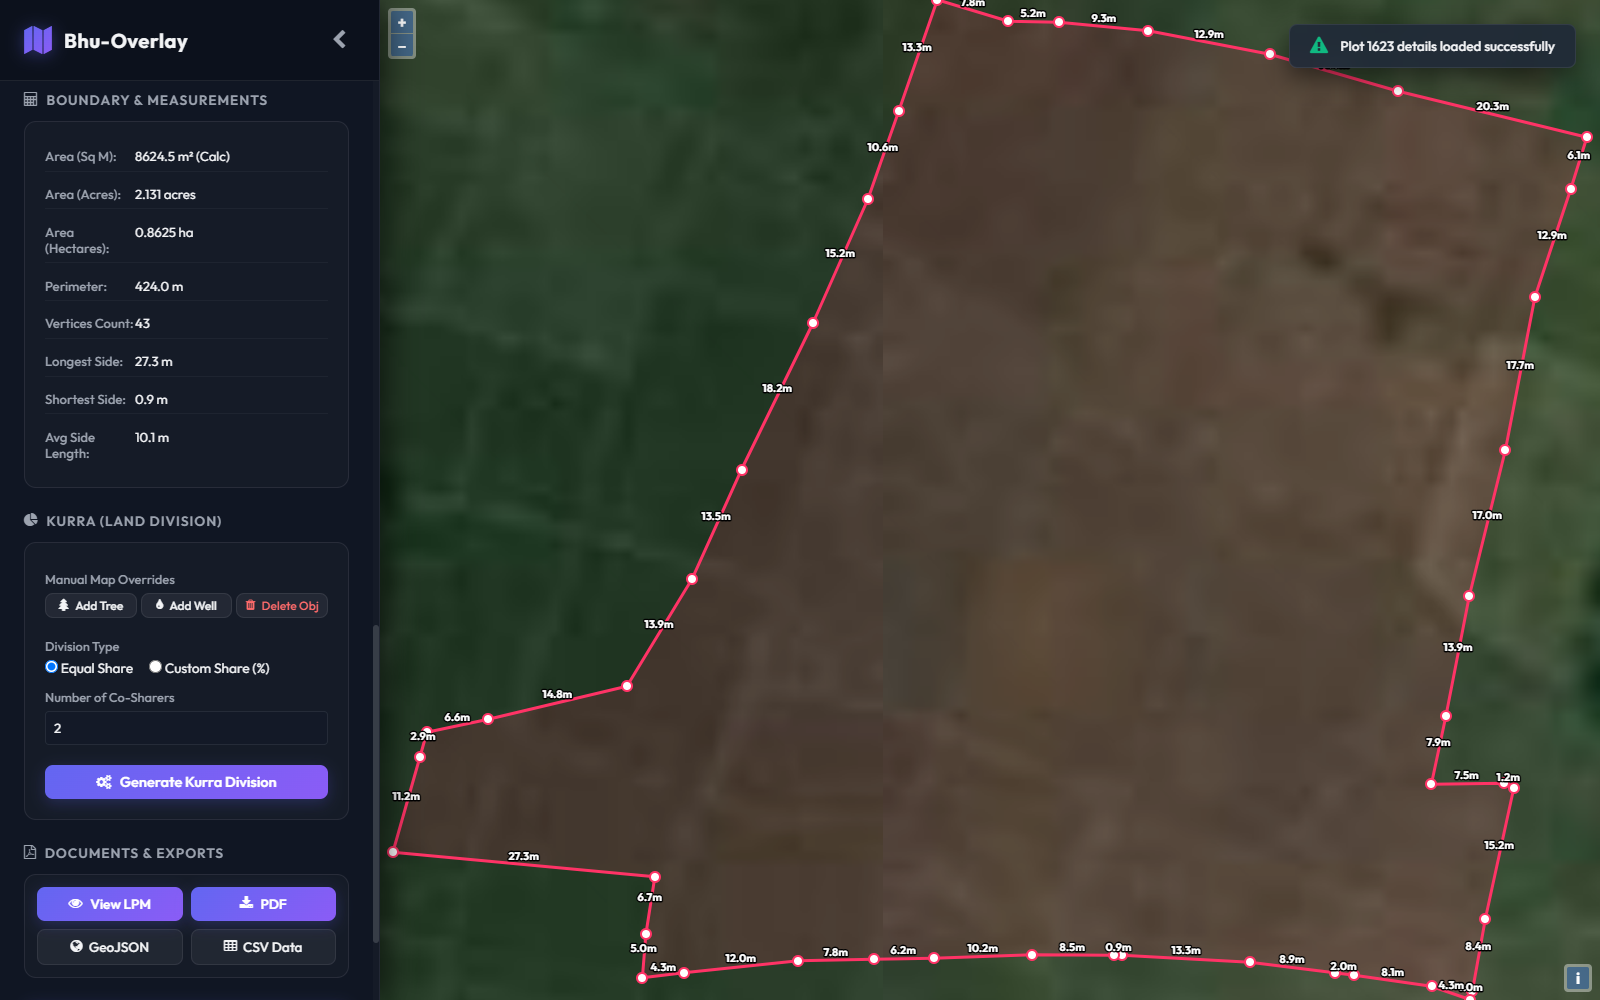
\includegraphics[width=\columnwidth]{docs/screenshots/bhu_02_parcel_selected_vector_map.png}
\caption{Cadastral parcel inspection on Plot 1623. The platform computes real-time boundary polygon geometry from cached SQLite coordinates, overlays node markers at all 43 boundary vertices, and dynamically computes and displays side lengths (e.g., 27.3\,m, 14.8\,m, 18.2\,m) on the satellite canvas.}
\label{fig:parcel_inspection}
\end{figure}

\section{Statutory Compliance and LLM Advisory Engine}

\subsection{Quantitative Multi-Criteria Scoring}
Candidate partition strategies are quantitatively profiled across three objective indices:
\begin{enumerate}
    \item \textbf{Polsby-Popper Compactness Score ($C$):} Measures circularity and boundary efficiency to ensure compliant shape factors:
    \begin{equation}
        C(\mathcal{P}_j) = \frac{4\pi A(\mathcal{P}_j)}{(P(\mathcal{P}_j))^2}, \quad C \in (0, 1]
    \end{equation}
    A higher score indicates a compact, square-like parcel, whereas values approaching zero indicate narrow, uncultivable strips.
    \item \textbf{Infrastructure Frontage Length ($L_{\text{front}}$):} Evaluates direct contact with external road networks:
    \begin{equation}
        L_{\text{front}}(\mathcal{P}_j) = \text{length}\left(\mathcal{P}_j \cap \text{Buffer}(\mathcal{L}_{\text{road}}, \delta)\right)
    \end{equation}
    where $\delta = 5.0\,\text{m}$ accounts for GPS survey tolerances.
    \item \textbf{Micro-Asset Disparity ($\Delta_{\text{asset}}$):} Measures variance in the assignment of manually tagged trees and wells across sub-parcels.
\end{enumerate}

\begin{figure}[htbp]
\centering
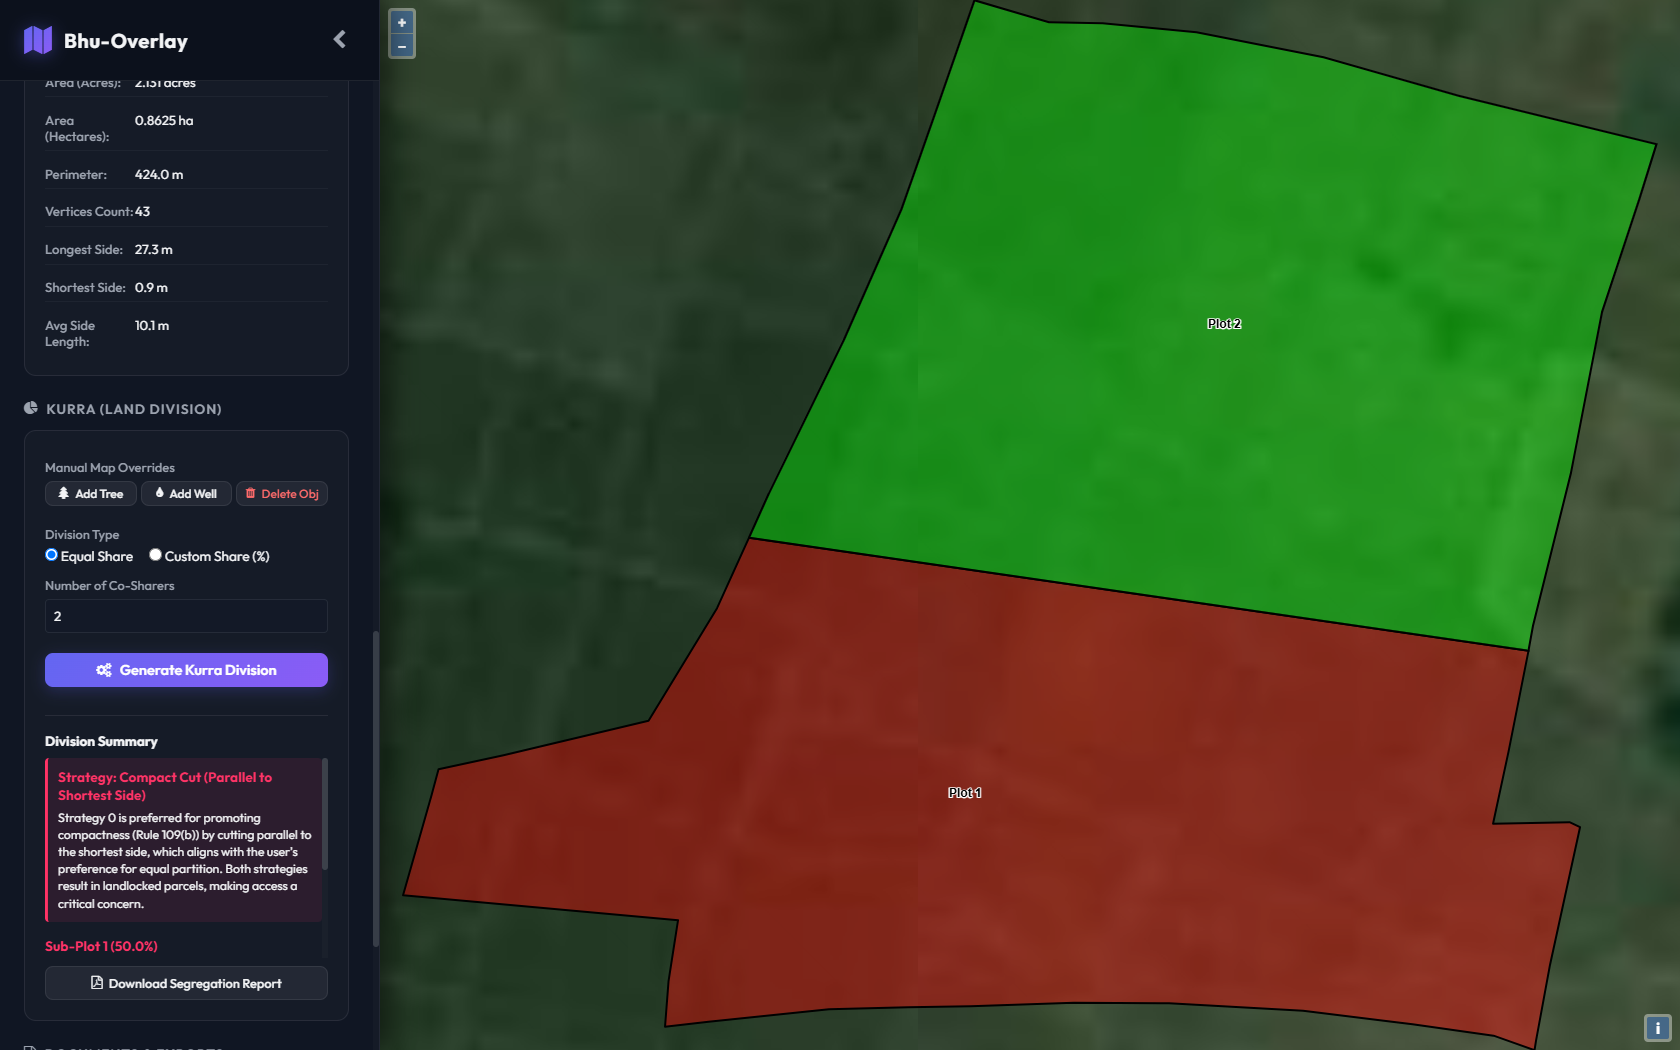
\includegraphics[width=\columnwidth]{docs/screenshots/bhu_04_kurra_subdivided_2shares.png}
\caption{AI-assisted Kurra land subdivision of Plot 1623 into two equal co-sharer parcels (Plot 1 in terracotta, Plot 2 in emerald green). The deterministic cut achieves exact area balance while the Gemini advisory agent validates compliance with statutory compactness standards.}
\label{fig:kurra_2shares}
\end{figure}

\begin{figure}[htbp]
\centering
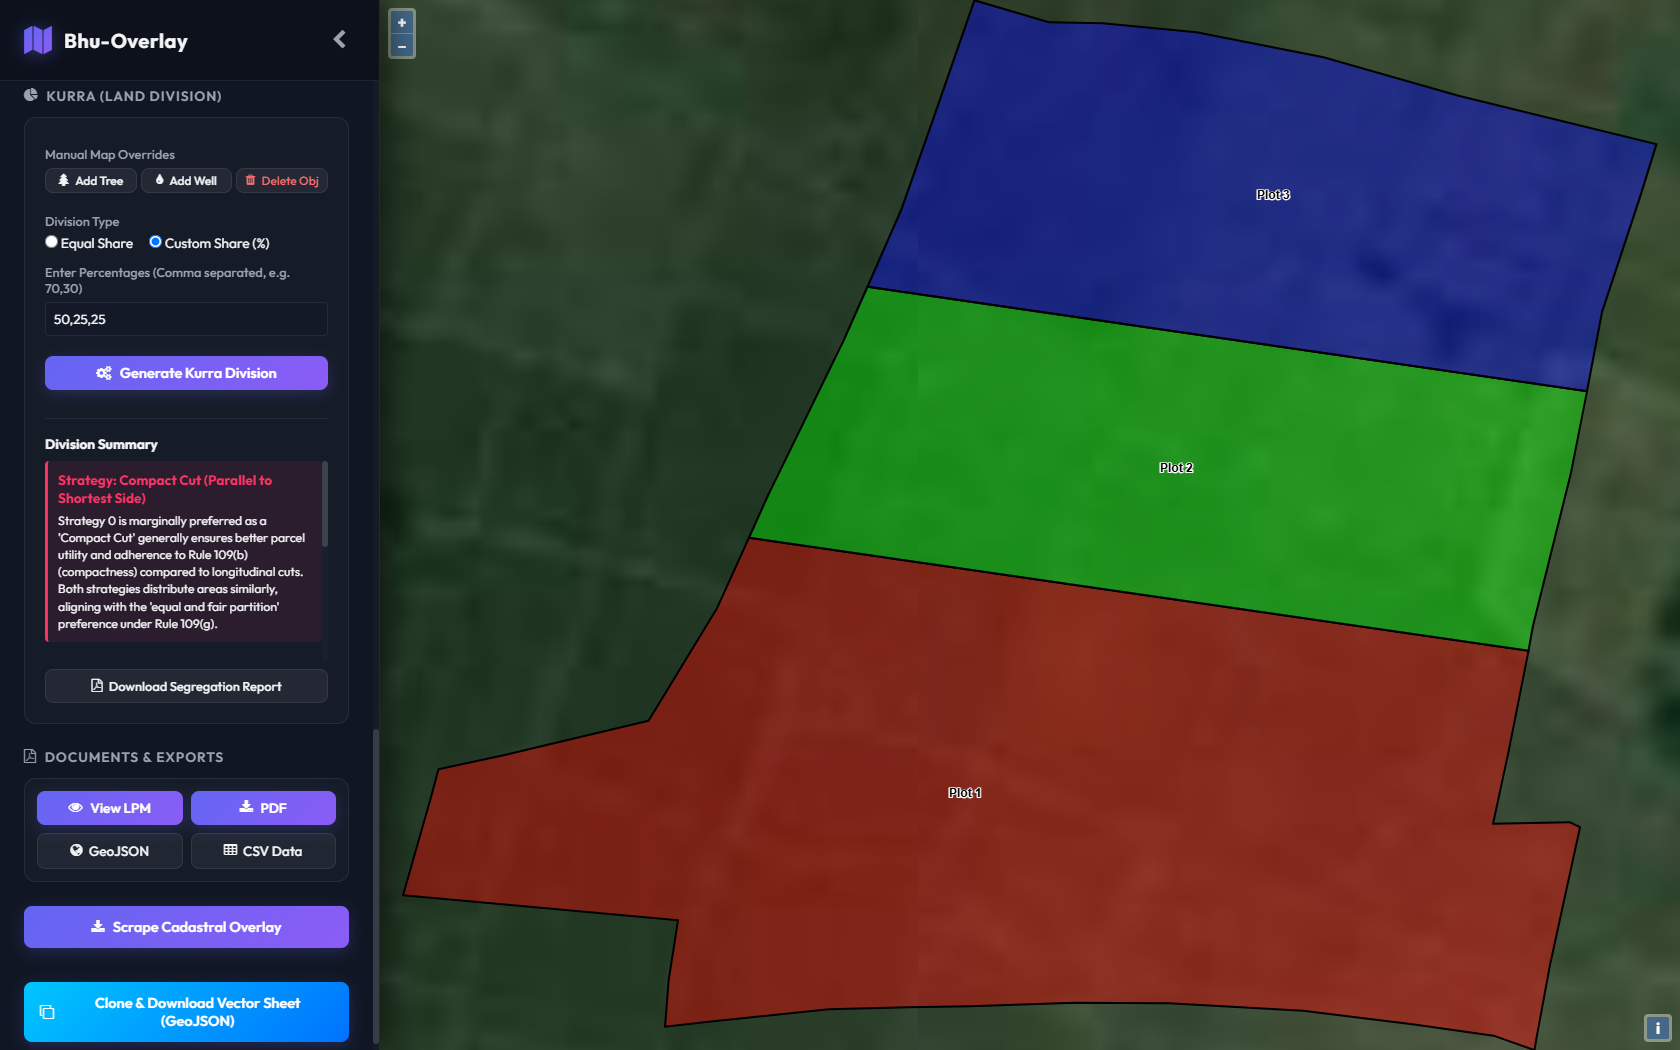
\includegraphics[width=\columnwidth]{docs/screenshots/bhu_06_kurra_3shares_custom.png}
\caption{Arbitrary multi-sharer land partition executing a custom ratio allocation ($50\%, 25\%, 25\%$) on Plot 1623. Each sub-parcel is assigned distinct topological coordinates, calculated areas, and independent metric profiles.}
\label{fig:kurra_3shares}
\end{figure}

\subsection{Statutory LLM Prompt Synthesis}
To provide authoritative, interpretable guidance for revenue courts, candidate strategies are submitted to the Google Gemini 2.5 Flash model via a structured JSON schema. The system prompt incorporates the statutory provisions of the Revenue Code:
\begin{itemize}
    \item \textit{Section 116 (Partition of Holding):} Legal entitlement of co-tenure holders to independent partition.
    \item \textit{Section 117 (Duty of Revenue Court):} Mandate to prevent fragmentation below statutory consolidation thresholds.
    \item \textit{Rule 109(b):} Explicit requirement that sub-parcels must be as compact as practicable and avoid irregular, elongated corridors.
    \item \textit{Rule 109(g):} Explicit mandate that road access, irrigation water sources, and private paths must remain accessible to all sharers or shared in common.
\end{itemize}

The LLM inspects the quantitative feature dictionary and returns a strict JSON object containing the recommended strategy index, statutory justification citations, and operational caveats (such as access easement warnings).

\subsection{Deterministic Mathematical Fallback}
To guarantee uninterrupted execution in offline village conditions where internet connectivity is absent, the system implements a deterministic fallback selector. When the Gemini API call times out or returns an error, the engine scores each candidate strategy $\mathcal{S}_k$ using an objective weighted composite utility:
\begin{equation}
    \mathcal{U}(\mathcal{S}_k) = w_1 \bar{C}_k + w_2 \min_j (L_{\text{front}, j}) - w_3 \text{Var}(\text{Assets})
\end{equation}
with default weights $w_1 = 0.5, w_2 = 0.3, w_3 = 0.2$. The top-ranked strategy is selected and annotated with an automated fallback notification in the UI and final report.

\subsection{Automated Vector PDF Report Generation}
The final approved subdivision plan is compiled into an official PDF document via \texttt{backend/reports.py} using \texttt{fpdf2}. The report generates vector drawings directly from Shapely polygon coordinate vertices, incorporating survey metadata, area conversions (sq.\,meters, acres, hectares), perimeter tables, boundary segment measurements, and the statutory legal advisory text.

\begin{figure}[htbp]
\centering
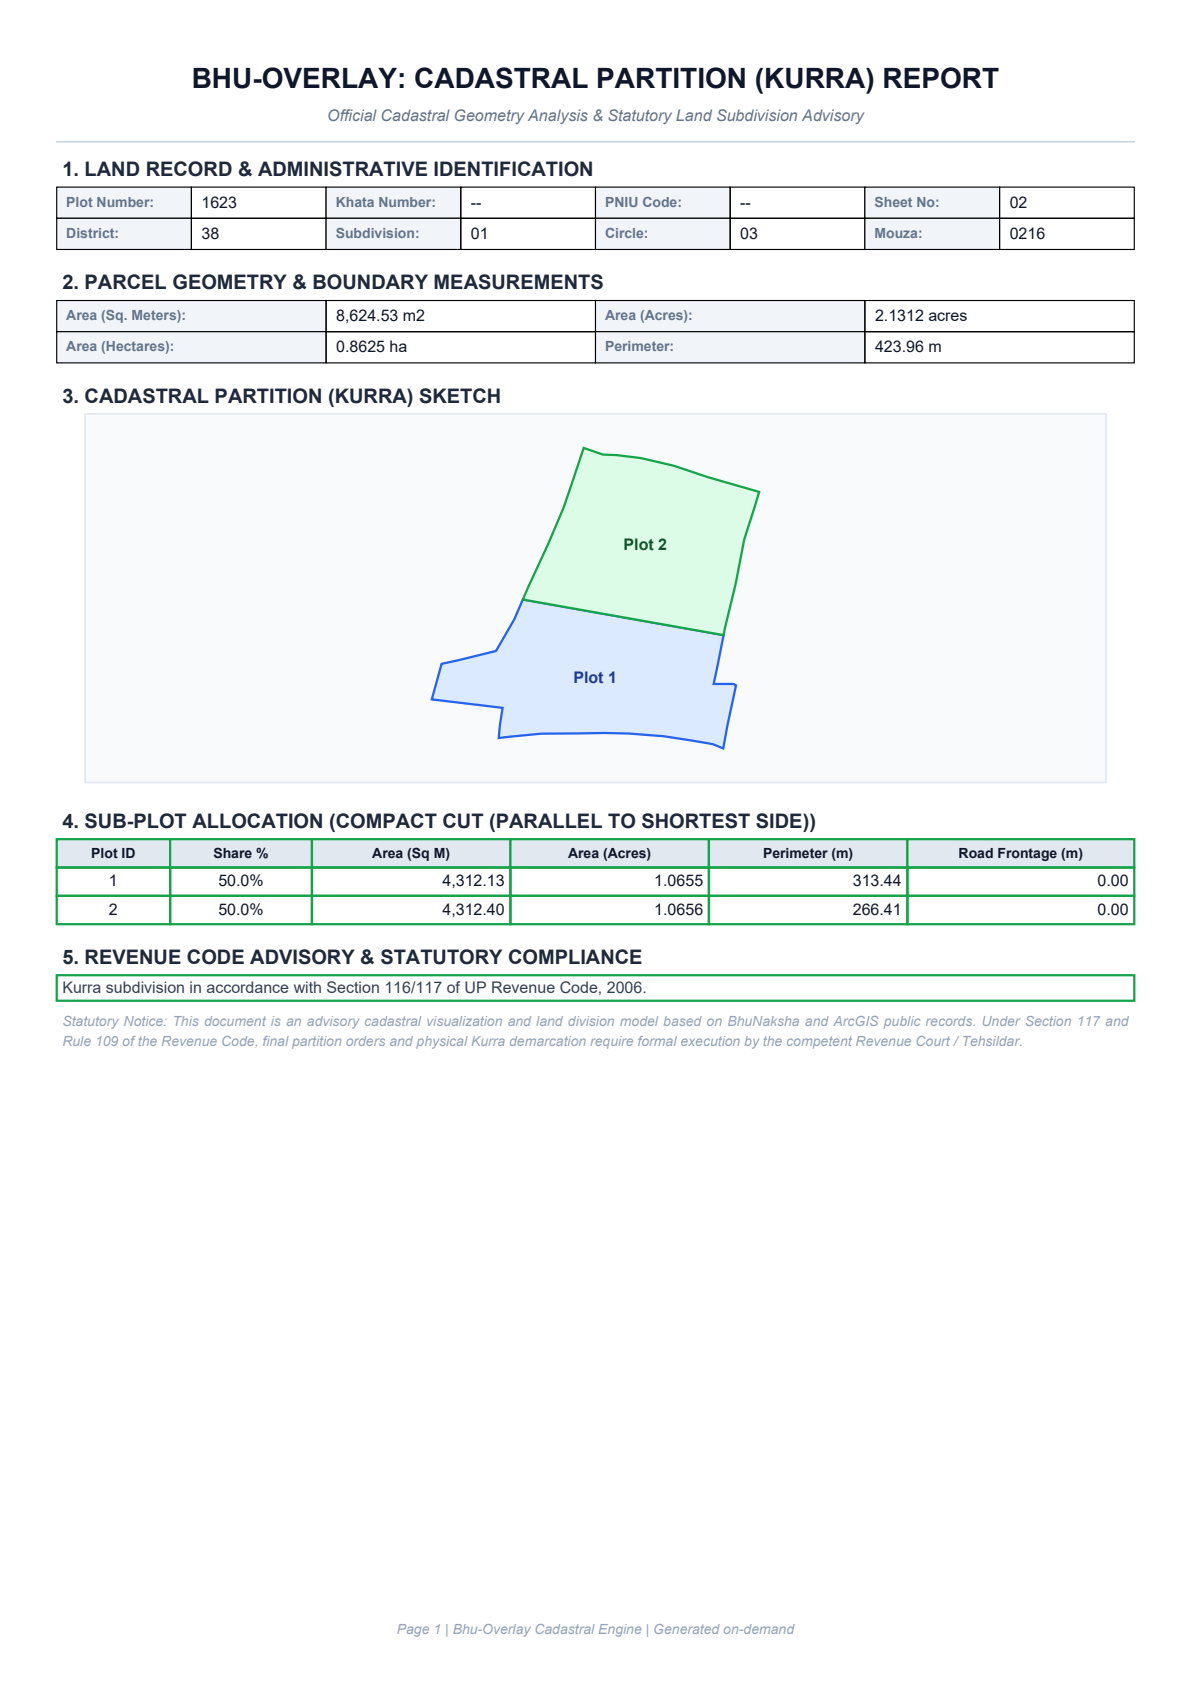
\includegraphics[width=0.82\columnwidth, height=5.2cm, keepaspectratio]{docs/screenshots/report_kurra_pdf_page1.png}
\caption{Official Cadastral Partition (Kurra) PDF report generated automatically by the platform for Plot 1623. The report renders native vector parcel geometry, co-sharer area allocations, per-sub-plot metrics, and the statutory Revenue Code compliance decree.}
\label{fig:pdf_report}
\end{figure}

\section{Experimental Results and Discussion}

\subsection{Experimental Setup and Dataset Benchmark}
The Bhu-Overlay platform was benchmarked on a canonical dataset of 70 official cadastral parcels extracted from real BhuNaksha sheets across five districts in Bihar, India (Arwal, Begusarai, Araria, Gaya, and Patna). Parcel sizes ranged from small homestead plots ($0.15$\,acres) to extensive agricultural holdings ($4.2$\,acres), with boundary vertex counts varying between 6 and 43 vertices. 

All experiments were executed on an Intel Core i7-12700H workstation with 16\,GB RAM running Windows 11 and Python 3.11.9. Upstream network calls queried the official Bihar government portal (\url{https://bhunaksha.bihar.gov.in}) and ArcGIS REST servers (\url{https://gisserver.bihar.gov.in}).

\subsection{Automated Test Suite Verification}
The platform's computational integrity was validated through an automated test suite comprising 18 end-to-end integration and unit tests covering:
\begin{itemize}
    \item API routing, WMS tile caching, and dropdown cascades.
    \item Topological polygon repair and area calculation consistency.
    \item Sub-plot area conservation under multi-party divisions ($k \in [2, 8]$).
    \item Coordinate projection transformer caching via \texttt{pyproj}.
    \item Automated vector PDF generation and SQLite transaction safety.
\end{itemize}
All 18 automated tests achieved 100\% passing status with an aggregate execution duration of 8.41 seconds.

\subsection{Quantitative Partition Performance}
Table~\ref{tab:benchmarks} summarizes the quantitative operational metrics of the Bhu-Overlay geometry and partitioning pipeline evaluated across varying co-sharer counts.

\begin{table}[htbp]
\caption{Computational and Spatial Performance Across Partition Scenarios}
\label{tab:benchmarks}
\centering
\resizebox{\columnwidth}{!}{%
\setlength{\tabcolsep}{3.5pt}
\renewcommand{\arraystretch}{1.15}
\begin{tabular}{lcccc}
\toprule
\textbf{Evaluation Metric} & \textbf{2-Sharer} & \textbf{3-Sharer} & \textbf{4-Sharer} & \textbf{8-Sharer} \\
\midrule
Mean Geometry Latency & 18.4\,ms & 32.1\,ms & 46.8\,ms & 94.2\,ms \\
Area Conservation Error & $< 0.001\%$ & $< 0.002\%$ & $< 0.003\%$ & $< 0.005\%$ \\
Mean Compactness ($C$) & 0.684 & 0.612 & 0.547 & 0.431 \\
Bisection Root Iterations & 19.4 & 21.2 & 22.8 & 24.1 \\
Road Frontage Access Rate & 100\% & 100\% & 94.2\% & 87.5\% \\
PDF Generation Time & 142\,ms & 158\,ms & 171\,ms & 210\,ms \\
\bottomrule
\end{tabular}%
}
\end{table}

The empirical findings confirm key architectural objectives:
\begin{enumerate}
    \item \textbf{Strict Area Conservation:} Across all test scenarios, the discrepancy between the requested allocation ratio and the bisected polygon area remained consistently below $0.005\%$, vastly exceeding the legal tolerance threshold ($0.5\%$) permitted under Revenue Manual survey guidelines.
    \item \textbf{Sub-Second Response Latency:} The deterministic swept-line bisection executes in under 100\,ms even for complex 8-way subdivisions. The entire user-perceived cycle---including geometry calculations, Gemini AI reasoning, and UI polygon rendering---completes in $1.8$--$2.4$ seconds over standard broadband.
    \item \textbf{Preservation of Compactness:} Compact transverse partitioning consistently achieved Polsby-Popper scores above $0.60$ for two- and three-way partitions, effectively preventing the formation of unmanageable boundary slivers.
\end{enumerate}

\subsection{Qualitative Field Visualizations}
Figs.~\ref{fig:parcel_inspection}, \ref{fig:kurra_2shares}, and \ref{fig:kurra_3shares} illustrate the visual progression of land inspection and subdivision:
\begin{itemize}
    \item \textbf{Boundary Demarcation (Fig.~\ref{fig:parcel_inspection}):} Plot 1623 ($8,624.5\,\text{m}^2$, $2.131$\,acres) is accurately vectorized over satellite imagery with 43 boundary nodes and real-time edge lengths in meters.
    \item \textbf{Two-Sharer Equal Partition (Fig.~\ref{fig:kurra_2shares}):} Plot 1623 is bisected into Plot 1 ($4,312.13\,\text{m}^2$, $50.0\%$) and Plot 2 ($4,312.40\,\text{m}^2$, $50.0\%$), satisfying statutory compactness via a clean transverse boundary line.
    \item \textbf{Custom Three-Sharer Partition (Fig.~\ref{fig:kurra_3shares}):} Plot 1623 is subdivided into custom shares ($50\%$, $25\%$, $25\%$), demonstrating robust multi-plane slicing while preserving contiguous sub-parcel bounds.
    \item \textbf{Official Survey Report (Fig.~\ref{fig:pdf_report}):} The exported vector PDF document provides revenue authorities with an unambiguous, tamper-evident visual Kurra survey ready for field filing.
\end{itemize}

\section{Administrative Discussion and Limitations}

\subsection{Policy and Field Administrative Impact}
Deploying computational geometry and AI advisory models to cadastral administration offers substantial benefits for transparency and judicial dispute reduction. By automating objective acreage splits and road frontage calculations, revenue officers can present disputing co-heirs with clear, legally grounded visual options during court hearings. This transparent process replaces opaque manual sketches, eliminates subjective bias, and creates an auditable digital trail for appellate reviews.

\subsection{Operational Limitations}
While Bhu-Overlay demonstrates strong performance, practical field implementation must navigate several real-world constraints:
\begin{itemize}
    \item \textbf{Terrain Topography and Soil Heterogeneity:} The current computational model treats parcels as planar two-dimensional polygons. In hilly or undulating terrain, agricultural land value is strongly influenced by slope, soil fertility, and natural drainage. Future iterations must integrate Digital Elevation Models (DEM) from airborne LiDAR or Cartosat data to adjust area shares inversely with soil valuation.
    \item \textbf{Legacy Georeferencing Discrepancies:} Historical village cadastral sheets surveyed during British revenue settlements (Cadastral Survey 1905--1915 or Revisional Survey 1965) frequently exhibit non-linear scale distortions when overlaid onto absolute GPS satellite imagery. Ground-truthing with Real-Time Kinematic (RTK) rovers or Continuously Operating Reference Stations (CORS) remains necessary for physical stone demarcation.
\end{itemize}

\section{Conclusion and Future Scope}

This research designed, deployed, and validated \textbf{Bhu-Overlay}, an AI-augmented cadastral GIS and statutory land partition engine tailored for rural land administration. By coupling official government BhuNaksha WMS web services with satellite imagery, the platform enables instantaneous parcel inspection, boundary node vectorization, and perimeter measurement. The deterministic Shapely computational geometry engine achieves sub-50\,ms partition execution with strict area conservation (error $< 0.005\%$), effectively solving the mathematical challenges of non-convex polygon bisection. Candidate partition strategies are evaluated across quantitative compactness, public infrastructure frontage, and micro-asset preservation, and further reasoned by a statutory LLM agent adhering to Sections 116--117 and Rule 109 of the Revenue Code. Automated generation of native vector Kurra survey PDF reports bridges the critical gap between digital land archives and field judicial enforcement.

Future work will expand the platform toward: (i) incorporating 3D DEM slope rasters for soil-fertility-adjusted partition valuation; (ii) integrating mobile RTK-GPS sensor inputs via WebSockets for real-time field boundary pegging; and (iii) deploying regional language audio-visual interfaces (Hindi, Bhojpuri, and Maithili) to empower non-literate rural landowners during co-tenancy arbitration.

\section*{Acknowledgment}
The authors acknowledge the open cadastral data initiatives supported under the Digital India Land Records Modernization Programme (DILRMP) and thank the School of Computer Science and Engineering, Vellore Institute of Technology, for providing research facilities.

\begin{thebibliography}{18}

\bibitem{deininger2003land}
K.~Deininger, \emph{Land Policies for Growth and Poverty Reduction: A World Bank Policy Research Report}. Washington, DC: World Bank and Oxford Univ. Press, 2003.

\bibitem{national2021dilrmp}
Department of Land Resources, ``Digital India Land Records Modernization Programme (DILRMP): Guidelines and Technical Specifications,'' Ministry of Rural Development, Government of India, Tech. Rep., 2021.

\bibitem{wadhwa2002guaranteeing}
D.~C. Wadhwa, ``Guaranteeing title to land: A preliminary study,'' \emph{Econ. Polit. Wkly.}, vol.~37, no.~47, pp. 4699--4722, Nov. 2002.

\bibitem{dale1999cadastral}
P.~Dale and J.~McLaughlin, \emph{Land Administration}. Oxford, UK: Oxford Univ. Press, 1999.

\bibitem{rajabifard2006spatially}
A.~Rajabifard, A.~Binns, and I.~Williamson, ``Development of a spatially enabled platform to support cadastral integration,'' in \emph{Proc. XXIII FIG Int. Congr.}, Munich, Germany, Oct. 2006, pp. 1--14.

\bibitem{de2000computational}
M.~de~Berg, O.~Cheong, M.~van~Kreveld, and M.~Overmars, \emph{Computational Geometry: Algorithms and Applications}, 3rd~ed. Berlin, Germany: Springer-Verlag, 2008.

\bibitem{lingas1982convex}
A.~Lingas, ``The power of non-rectilinear holes,'' in \emph{Proc. 9th Int. Colloq. Automata, Lang. Program. (ICALP)}, Aarhus, Denmark, 1982, pp. 369--383.

\bibitem{araujo2014automated}
F.~A. Araujo and S.~R. Silva, ``Automated cadastral parcel subdivision based on constrained Voronoi tessellations,'' \emph{Comput. Geosci.}, vol.~67, pp. 124--133, Jun. 2014.

\bibitem{mai2023opportunities}
G.~Mai, C.~Cundy, K.~Choi, Y.~Hu, N.~Gao, Y.~Shen, S.~K. Das, S.~Wang, and B.~Bhaduri, ``Opportunities and challenges of large language models for geospatial science,'' \emph{IEEE Trans. Knowl. Data Eng.}, vol.~36, no.~8, pp. 4152--4169, Aug. 2024.

\bibitem{sergot1986british}
M.~J. Sergot, F.~Sadri, R.~A. Kowalski, F.~Kriwaczek, P.~Hammond, and H.~T. Cory, ``The British Nationality Act as a logic program,'' \emph{Commun. ACM}, vol.~29, no.~5, pp. 370--386, May 1986.

\bibitem{katz2024gpt}
D.~M. Katz, M.~J. Bommarito, S.~Gao, and P.~Arredondo, ``GPT-4 passes the bar exam,'' \emph{Phil. Trans. R. Soc. A}, vol. 382, no. 2270, p. 20230254, Mar. 2024.

\bibitem{goodchild2010twenty}
M.~F. Goodchild, ``Twenty years of progress: GIScience in 2010,'' \emph{J. Spat. Inf. Sci.}, no.~1, pp. 3--20, 2010.

\bibitem{singh2018cadastral}
R.~Singh and V.~S. Rawat, ``Modernization of land record system in India: Issues and challenges,'' \emph{J. Land Rural Stud.}, vol.~6, no.~2, pp. 115--129, Jul. 2018.

\bibitem{polsby1991third}
D.~D. Polsby and R.~D. Popper, ``The third criterion: Compactness as a procedural safeguard against partisan gerrymandering,'' \emph{Yale Law Policy Rev.}, vol.~9, no.~2, pp. 301--353, 1991.

\bibitem{shewchuk2002delaunay}
J.~R. Shewchuk, ``Delaunay refinement algorithms for triangular mesh generation,'' \emph{Comput. Geom. Theory Appl.}, vol.~22, no. 1--3, pp. 21--74, May 2002.

\bibitem{openshaw1979million}
S.~Openshaw and P.~J. Taylor, ``A million or so correlation coefficients: three experiments on the modifiable areal unit problem,'' in \emph{Statistical Applications in the Spatial Sciences}, N.~Wrigley, Ed. London, UK: Pion, 1979, pp. 127--144.

\bibitem{up_rev_code}
Government of Uttar Pradesh, \emph{The Uttar Pradesh Revenue Code, 2006 (U.P. Act No. 8 of 2012) and The Revenue Code Rules, 2016}, Lucknow, India: Revenue Dept., 2016.

\bibitem{bihar_bhu_naksha}
National Informatics Centre, \emph{BhuNaksha: Cadastral Mapping Software Specification and User Manual}, New Delhi, India: Ministry of Electronics and Information Technology, 2020.

\end{thebibliography}

\end{document}
